\documentclass[letterpaper]{article}
\usepackage[utf8]{inputenc}
\usepackage[spanish, mexico]{babel}
\usepackage{amssymb, amsmath}
\usepackage{stackengine}
\usepackage{graphicx}
\usepackage{ mathrsfs }
\usepackage{lipsum}
\usepackage{dsfont}
\usepackage[margin=1.5cm,
vmargin={1.5cm,0.7cm},
includefoot]{geometry}
\usepackage{setspace}
\usepackage{subcaption}
\usepackage{tocloft}
\usepackage{upgreek}
\usepackage{amsthm}
\usepackage{graphicx}
\usepackage{paralist}
\usepackage{fancyhdr}
\usepackage{lmodern}
\usepackage{tcolorbox}
\usepackage{color}
\usepackage{tikz}
\usepackage{wasysym}
\usepackage{textgreek, marvosym}
\tcbuselibrary{skins,breakable}
\pagestyle{fancy}

\renewcommand{\headrulewidth}{0.4pt}
\renewcommand{\footrulewidth}{0.4pt}

\renewcommand{\d}{\partial}

\providecommand{\abs}[1]{\left|#1\right|}
\providecommand{\norm}[1]{\left|\left|#1\right|\right|}														  
\providecommand{\pint}[1]{\langle#1\rangle}														  
\newcommand{\V}{\mathds{V}}

\newcommand{\W}{\mathds{W}}

\newcommand{\F}{\mathds{F}}

\newcommand{\tq}{ \quad \cdot  \backepsilon \cdot \quad }

\newcommand{\ld}{\lim\limits_{x \to 0^{+}}}

\newcommand{\li}{\lim\limits_{x \to 0^{-}}}

\newcommand{\la}{\lim\limits_{x \to a}}

\renewcommand{\l}{\ell}

\newcommand{\R}{\mathds{R}}

\newcommand{\Po}{\mathds{P}_2(\mathds{R})}

\renewcommand{\*}{\cdot}

\makeatletter
\renewcommand*\env@matrix[1][\arraystretch]{%
	\edef\arraystretch{#1}%
	\hskip -\arraycolsep
	\let\@ifnextchar\new@ifnextchar
	\array{*\c@MaxMatrixCols c}}
\makeatother

\newtheorem{theorem}{Teorema}[]
\theoremstyle{definition}
\newtheorem{definition}{Definición}


\begin{document}
	
	\setlength{\unitlength}{1cm}
	\thispagestyle{empty}
	\begin{picture}(19,3)
	\put(-0.5,1.2){
\includegraphics[scale=.20]{img/unam1.png}}
	\put(16,1){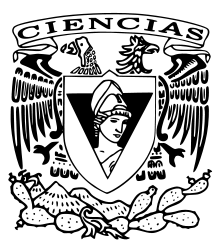
\includegraphics[scale=.29]{img/fciencias1.png}}
	\end{picture}
	
	\begin{center}
		\vspace{-114pt}
		\textbf{\large Matemáticas para las Ciencias II}\\
		\textbf{ Semestre 2020-2}\\
		Prof. Pedro Porras Flores\\
		Ayud. Irving Hernández Rosas \\
		\textbf{Tarea Examen II}\\[0.15cm]
		Kevin Ariel Merino Peña\footnote{Número de cuenta 317031326}\\ [0.12cm]
		\today
	\end{center}
	\vspace{-10pt}
	\rule{19cm}{0.3mm}
	
\noindent Realice los siguientes ejercicios, escribiendo el procedimiento claramente. Y recuerden la tarea-examen se entregan de manera individual.\\
\noindent1. El volumen específico $ V $, la presión $ P $  la temperatura $ T $ de un gas van der Waals están relacionados por
\[ P = \dfrac{RT}{V - \beta} - \dfrac{\alpha}{V^2} \] donde $ \alpha, \beta $ y $ R $ son constantes.\\

a) Encuentre $ \dfrac{\d T}{\d P}, \dfrac{\d P}{\d V} $ y $ \dfrac{\d V}{\d T} $.\\

Consideremos lo siguiente en función de la temperatura y el volumen como 
\[ P(T,V) = \dfrac{RT}{V - \beta} - \dfrac{\alpha}{V^2} \label{eq:uno}\tag{1} \]
observemos que la ecuación anterior tiene al menos una solución tal que $ P(T,V) = 0 $ pues como $ \alpha  $ es una constante podemos elegirla cero  y $ R $ o $ T $ iguales a cero, (alguna otra podría ser que entre ambos sumandos se hagan inversos aditivos.Como cada variable puede ser considerada independiente entonces, podemos proceder a despejar $ T $ com variable independiente
\begin{align*}
	P &= \dfrac{RT}{V - \beta} - \dfrac{\alpha}{V^2} &&\text{Por la primera ecuación en el ejercicio}\\
	P - \dfrac{RT}{V - \beta}&=  - \dfrac{\alpha}{V^2} &&\text{sumando en ambos miembros el inverso aditivo de } \dfrac{RT}{V - \beta}\\
	- \dfrac{RT}{V - \beta}&= -P - \dfrac{\alpha}{V^2} &&\text{sumando en ambos miembros el inverso aditivo de } P\\
	\dfrac{RT}{V - \beta}&= P + \dfrac{\alpha}{V^2} &&\text{Multiplicando ambos miembros por} -1\\
	RT&= \left(P + \dfrac{\alpha}{V^2}\right) (V - \beta) &&\text{Multiplicando ambos miembros por el inverso multiplicativo de } V - \beta\\
	T&= \left(P + \dfrac{\alpha}{V^2}\right) (V - \beta) \dfrac{1}{R} &&\text{Multiplicando ambos miembros por } \dfrac{1}{R}\\
	T&= \left(P + \dfrac{\alpha}{V^2}\right) \dfrac{V - \beta}{R} &&\text{Reescribiendo la ecuación}\\
	T (V,P)&= \left(P + \dfrac{\alpha}{V^2}\right) \dfrac{V - \beta}{R} &&\text{Poniéndola en función de las variables}
\end{align*}
\[ T(V,P) = \left( P + \dfrac{\alpha}{V^2} \right) \dfrac{V - \beta}{R} \label{eq:dos}\tag{2} \]

Por otro lado, es importante hacer una tercera observación
\begin{align*}
	P &= \dfrac{RT}{V - \beta} - \dfrac{\alpha}{V^2} &&\text{Por la primera ecuación en el ejercicio}\\
	P &=  \dfrac{RTV^2-\alpha(V- \beta)}{V^2(V - \beta)} &&\text{Empleando la regla de suma de fracciones}\\
	V^2(V - \beta)P &=  RTV^2-\alpha(V- \beta) &&\text{Multiplicando ambos miembros por }V^2(V - \beta)\\
	(V^3 - V^2\beta)P &=  RTV^2-\alpha(V- \beta) &&\text{Desarrolando el primer miembros por distributividad}\\
\end{align*}
\[ (V - \beta)V^2 P = RTV^2 - \alpha(V - \beta) \label{eq:tres}\tag{3}  \]

Empleando las dos observaciones anteriores podemos ver que
\begin{align*}
	\dfrac{\d T}{\d P} &= \dfrac{V - \beta}{R} &&\text{Por la segunda observación, donde despejamos }T \label{eq:cuatro}\tag{4} \\
	\dfrac{\d P}{\d V} &= \dfrac{-RT}{(V - \beta)^2}  + \dfrac{2\alpha}{V^3}&&\text{Por la función original} \label{eq:cinco}\tag{5} \\\
\end{align*}
Para obtener la derivada del volumen con respecto a la temperatura, tomemos a $ P $ como una constante y derivemos con respecto a $ T $ obtenemos:
\begin{align*}
(V - \beta)V^2 P &= RTV^2 - \alpha(V - \beta) &&\text{Por la ecuación (\ref{eq:tres})}\\
(V - \beta)V^2 P + \alpha(V - \beta) &= RTV^2 &&\text{Sumando en ambos miembros }\alpha(V - \beta)\\
(V - \beta)V^2 P + \alpha\dfrac{(V - \beta)}{V^2} &= RT &&\text{Multiplicando ambos miembros por }\dfrac{1}{V^2}\\
(V - \beta)V^2 P + \alpha\dfrac{(V - \beta)}{V^2} - RT &= 0 &&\text{Igualando a } 0
\end{align*}
\begin{align*}
	F(V,T) &= (V - \beta)V^2 P + \alpha\dfrac{(V - \beta)}{V^2} - RT &&\text{Definamos una nueva función auxiliar como sigue}\\
	\dfrac{\d }{\d V}F(V,T) &= (V - \beta)V^2 P + \alpha\dfrac{(V - \beta)}{V^2} - RT &&\text{Calculemos la derivada parcial con respecto a }V\\
	\dfrac{\d }{\d V}F(V,T) &= P + \alpha\left(\dfrac{\d}{\d V}\left(\dfrac{1}{V^2}\right) - \dfrac{\d}{\d V}\left(\dfrac{\beta}{V^2}\right) \right) &&\text{Calculemos la derivada parcial con respecto a }V\\
	\dfrac{\d }{\d V}F(V,T) &= P + \alpha\left(\dfrac{-V + 2\beta}{ V^3 } \right) &&\text{Calculemos la derivada parcial con respecto a }V\\
	\\
	\dfrac{\d }{\d T}F(V,T) &= (V - \beta)V^2 P + \alpha\dfrac{(V - \beta)}{V^2} - RT &&\text{Calculemos la derivada parcial con respecto a T}\\
	\dfrac{\d }{\d T}F(V,T) &= -R &&\text{Pues el únco término con T} era -RT\\
\end{align*}
Luego, recordemos por un teorema visto en Mate I que 
$ \dfrac{\d V}{\d T} = - \dfrac{F_T(V,T)}{F_V(V,T)} $, entonces tenemos que 
\begin{align*}
	\dfrac{\d V}{\d T} &= - \dfrac{-R}{ P + \alpha\left( \dfrac{-V + 2\beta}{V^3} \right) } &&\text{Por el teorema de Cálculo I}\\
	\dfrac{\d V}{\d T} &=  \dfrac{R}{ \dfrac{RT}{V - \beta} - \dfrac{\alpha}{V^2}  + \alpha\left( \dfrac{-V + 2\beta}{V^3} \right) } &&\text{Por cómo definimos }P\\
	\dfrac{\d V}{\d T} &=  \dfrac{R}{ (V - \beta) \left(\dfrac{RT}{(V - \beta)^2} - \dfrac{2\alpha}{V^3}\right)} &&\text{Simplificando }\\
\end{align*}


Identifique qué variables son constantes e interprete físicamente cada derivada parcial.\\

En $ (\ref{eq:cuatro}) $ tenemos que si $ R > 0 $, entonces $ \dfrac{\d T}{\d P} $ también será postivia, esto significa que la temperatura $ T $ está creciendo con respecto a la presión $ P $ cuando el volúmen $ V $ es $ V > \beta $ y ésta disminuirá en otro caso. Cuando $ R<0 $ lo contrario ocurre.\\

Luego, por $ (\ref{eq:cinco}) $ podemos vemis que $ \dfrac{\d P}{\d V} > 0$ si $ \dfrac{RT}{(V - \beta)^2} > \dfrac{2\alpha}{V^3} $, lo que significa que la presión $ P $ crecerá con respecto al volumen $ V $. Además, entre más crezca $ V $ el volúmen, la presión se volverá cada vez más grande, vemos que si $ \dfrac{\d P}{\d V}  $ tiende a 0 es porque la presión se vuelve muy cercana a una constante (cuando incrementamos el volumen $ V $).

b) Verifique $ \left( \dfrac{\d T}{\d P}\right) \left( \dfrac{\d P}{\d V}\right)\left( \dfrac{\d V}{\d T}\right) = -1 $\\

Primero veamos que tenemos una manera distinta de escribir a $ (\ref{eq:cinco}) $ (haciendo la suma de fracciones)  como:
\[ \dfrac{\d P}{\d V} = \dfrac{-RTV^3 + 2\alpha(V - \beta)^2}{V^3(V-\beta)^2} \]
ahora tomemos $ (\ref{eq:cuatro}),(\ref{eq:cinco}) $ y la ultimoa ecuación reescrita para hacer el siguiente producto

\begin{align*}
	\dfrac{\d T}{\d P}\dfrac{\d P}{\d V}\dfrac{\d V}{\d T} &= \left( \dfrac{(V - \beta)}{R}\right)\* \left(\dfrac{-RTV^3 + 2\alpha(V - \beta)^2}{V^3(V-\beta)^2}\right)\* \left(\dfrac{R}{(V - \beta)\left(\dfrac{RT}{(V - \beta)^2} - \dfrac{2\alpha}{V^3}\right) }\right)\\
	\dfrac{\d T}{\d P}\dfrac{\d P}{\d V}\dfrac{\d V}{\d T}&= \left(V - \beta \right)\* \left(\dfrac{-RTV^3 + 2\alpha(V - \beta)^2}{V^3(V-\beta)^2}\right)\* \left(\dfrac{1}{(V - \beta)\left(\dfrac{RT}{(V - \beta)^2} - \dfrac{2\alpha}{V^3}\right) }\right)\\
	\dfrac{\d T}{\d P}\dfrac{\d P}{\d V}\dfrac{\d V}{\d T} &= \left(\dfrac{-RTV^3 + 2\alpha(V - \beta)^2}{V^3(V-\beta)^2} \right)\* \left(\dfrac{V - \beta }{(V - \beta)\left(\dfrac{RT}{(V - \beta)^2} - \dfrac{2\alpha}{V^3}\right) }\right)\\
	\dfrac{\d T}{\d P}\dfrac{\d P}{\d V}\dfrac{\d V}{\d T} &= \left(\dfrac{-RTV^3 + 2\alpha(V - \beta)^2}{V^3(V-\beta)^2} \right)\* \left(\dfrac{1}{\left(\dfrac{RT}{(V - \beta)^2} - \dfrac{2\alpha}{V^3}\right) }\right)\\ %%sera??
\end{align*}
\begin{align*}
	\dfrac{\d T}{\d P}\dfrac{\d P}{\d V}\dfrac{\d V}{\d T} &=  \dfrac{-RTV^3 + 2\alpha(V - \beta)^2 }{ V^3(V-\beta)^2 \left( \dfrac{RT}{(V - \beta)^2} - \dfrac{ 2\alpha }{ V^3 } \right) }\\
	\dfrac{\d T}{\d P}\dfrac{\d P}{\d V}\dfrac{\d V}{\d T} &=  \dfrac{-RTV^3 + 2\alpha(V - \beta)^2 }{ \dfrac{V^3(V - \beta)^2 RT }{(V - \beta)^2} - \dfrac{2V^3 \alpha(V - \beta)^2 }{V^3}}\\
	\dfrac{\d T}{\d P}\dfrac{\d P}{\d V}\dfrac{\d V}{\d T} &=  \dfrac{-RTV^3 + 2\alpha(V - \beta)^2 }{ V^3RT - 2\alpha(V - \beta)^2 }\\
	\dfrac{\d T}{\d P}\dfrac{\d P}{\d V}\dfrac{\d V}{\d T} &= -1\\
\end{align*}

\noindent2. Considere una función de temperatura $ T(x,y) = x\sin(y) $ Trazar algunas curvas de nivel. Calcula $ \nabla T $ y explique su significado.\\

Para trazar algunas curvas ade nivel, igualemos la función a alguna constante $ k $

\begin{align*}
	T(x,y) &= x\sin(y) &&\text{Ecuación dada}\\
	T(x,y) &= k &&\text{Para encontrar alguna curva de nivel}\\
	x\sin(y) &= k &&\text{Sustitiuyendo }T(x,y)\\
	\\
	x\sin(y) &= -1 &&\text{Evaluando en  }k < 0\\
	y &= \arcsin\left(-\dfrac{1}{x}\right) &&\text{Por cálculo I }\\
	\\
	x\sin(y) &= 2 &&\text{Evaluando en  }k > 0\\
	y &= \arcsin\left(\dfrac{2}{x}\right)&&\text{Por cálculo I }\\	
\end{align*}


Ahora calculemos el gradiente como $ \nabla T = \left(\dfrac{\d T}{\d x}, \dfrac{\d T}{\d y}\right) $, lo calculamos directamente:
\[ \nabla T(x,y) = (\sin(x), x\cos(y)) \]


\begin{figure}[h]
	\centering
	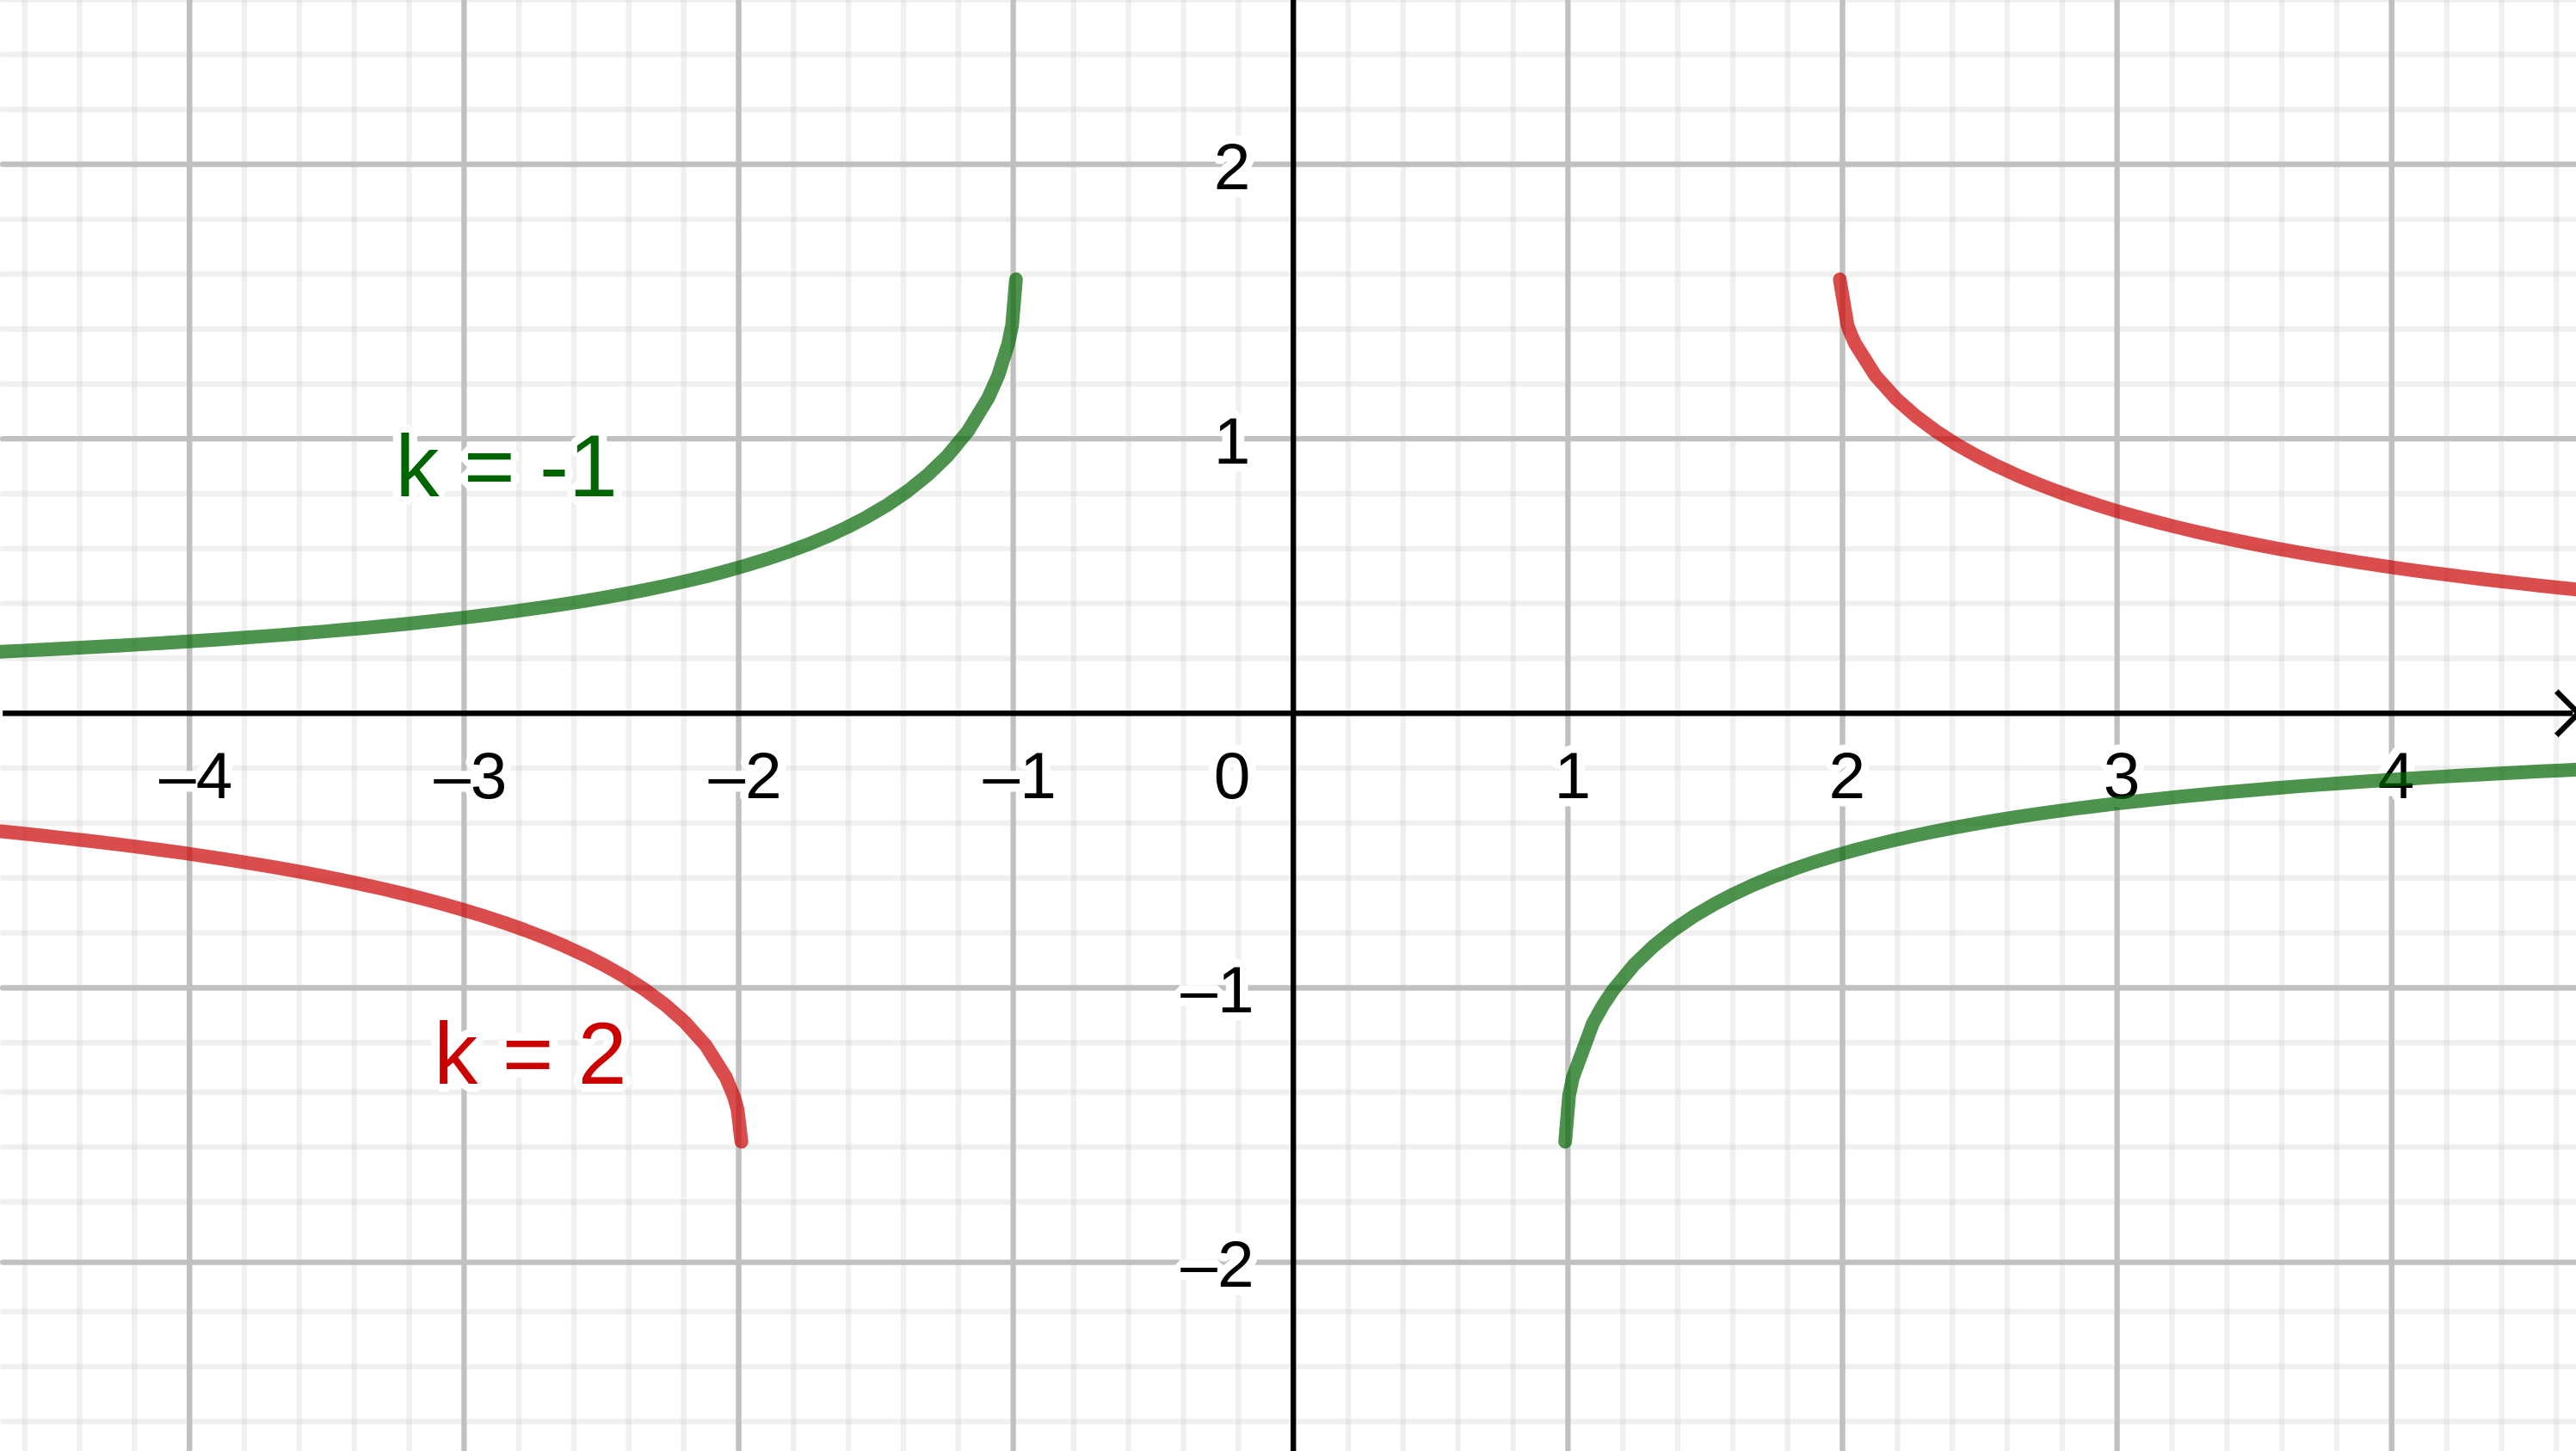
\includegraphics[height=0.3\textwidth]{img/ej2}
	\caption{En el plano, los cuadrantes 1 y 2, son el conjunto B}
\end{figure}

En todos los casos el gradiente nos ofrece la dirección de más rápido crecimiento en una función, en este caso habla sobre la dirección en que más rápido incrementa la temperatura.

\noindent3. Encuentre el plano tangente a la superficie $ z = x^2 + y^2 $ en el punto $ (1,-2,5) $. Explica el significado geométrico para esta superficie del gradiente de $ f(x,y)= x^2 + y^2 $\\

Observemos que el punto de interés es $ (x_0, y_0) = (1,-2) $, recordemos por clases anteriores, que el plano tangente a una función en el punto $ (x_0, y_0, f(x_0,y_0)) $ está dado por
\[ z = f(x_0, y_0) + \left[ \dfrac{\d f}{\d x}(x_0,y_0) \right] (x - x_0) + \left[ \dfrac{\d f}{\d y}(x_0, y_0)\right](y - y_0) \]
Ahora calculemos el gradiente
\begin{align*}
	\nabla f(x,y) &= \left( \dfrac{\d f}{\d x},\dfrac{\d f}{\d y} \right) && \text{Por definición de gradiente}\\
	\nabla f(x,y) &= \left( \dfrac{\d }{\d x} (x^2 + y^2),\dfrac{\d}{\d y} (x^2 + y^2) \right) && \text{Sustituyendo la función }\\
	\nabla f(x,y) &= \left( 2x, 2y \right) && \text{Evaluando las derivadas}\\
\end{align*}
luego calculemos el gradiente en el punto $(x_0, y_0) = (1,-2) $, esto es $ \nabla f(1,-2) = (2,-4) $, así podemos regresas a la ecuación del principio y sustituir
\[ z = 5+ 2(x - 1) - 4(y+2) \]
simplificando obtenemos la siguiente ecuación de un plano
\[ z = 2x -4y -5 \]
Además, sabemos que el gradiente nos ofrece la pendiente del plano tangente (con respecto a $ xy $) que está dado por $$ \norm{\nabla f(1,-2)} $$esto último es 
\begin{align*}
	\norm{\nabla f(1,-2)} &= \sqrt{2^2 + 4^2}\\
	\norm{\nabla f(1,-2)} &= 2\sqrt{5}
\end{align*}


\noindent4. Un bicho se encuentra en un entorno tóxico. El nivel de toxicidad está dado por $ T(x,y) = 2x^2 - 4y^2 $. Si el bicho está en $ (-1,2) $. ¿En qué dirección debería moverse para reducir la toxicidad más rápido.\\

Sabemos que la dirección de más rápido decrecimiento está dada por $ - \nabla T $ por los ejercicios hechos en el \textit{proyecto V} y teoremas probados en clase, entonces calculemos el gradiente de $ T $
\begin{align*}
	\nabla T (x,y) &= \left( \dfrac{\d T}{\d x}(x,y),\dfrac{\d T}{\d y}(x,y)  \right) &&\text{Por definición de gradiente}\\
	\nabla T (x,y) &= \left( 4x,-8y  \right) &&\text{Calculando las parciales}\\
	\\
	-\nabla T (-1,2) &= (4,16) &&\text{Sustituyendo el punto donde se encuentra el bicho}\\
\end{align*}
\begin{center}
	$ \therefore $ el bicho deberá moverse en dirección $ (4,16)$
\end{center}

\noindent5. El desplazamiento en el tiempo $ t $ y la posición horizontal en la recta $ x $ de una cierta cuerda de violín, está dada por $$ u(x,t) = \sin(x - 6t) + \sin(x+6t) $$ Calcule la velocidad de la cuerda en $ x = 1 $ cuando $ t = \dfrac{1}{3} $.\\
Estamos considerando el desplazamiento de la cuerda en $ x = 1 $, esto es una función 
\[ f(t) = u(1,t) = \sin(1-6t) + \sin(1 + 6t) \]
Entonces la velocidad (que es la derivada con respecto a la posición) está dada por $ f'(\frac{1}{3}) $, entonces calculemos la derivada de dicha función

\begin{align*}
	f(t) &= \sin(1-6t) + \sin(1 + 6t) && \text{Por la construcción de dicha función respecto al tiempo}\\
	f'(t) &= \dfrac{df}{dt}(\sin(1-6t)) + \dfrac{df}{dt}(\sin(1 + 6t)) && \text{Definición de la derivada}\\
	f'(t) &= -6\cos(1-6t) + \cos(1 + 6t) && \text{Calculando las derivadas}\\
	f'\left(\frac{1}{3}\right) &= -6\cos(1-6\left(\frac{1}{3}\right)) + \cos(1 + 6\left(\frac{1}{3}\right)) && \text{Evaluando en el tiempo dado}\\
	f'\left(\frac{1}{3}\right) &= 6(\cos(3)- \cos(1)) && \text{Simplificando (factorizando y usando la paridad del coseno)}\\
\end{align*}
\begin{center}
	Observemos que para cualqien $ x $ dado, el desplazamiento será estrictamente veritcal (se trata de una cuerda) puesto que sólo se mueve hacia arriba o abajo, así concluimos que el vector velocidad está dado por $ \vec{v} = (0,6(\cos(3) - \cos(1)) $
\end{center}

\noindent6. La altura $ h $ del volcán hawaiano Mauna Loa se describe (aproximadamente) por la función $$ H(x,y) = 2.59 - 0.00024y^2 - 0.00065x^2 $$donde $ h $ es la altura sobre el nivel del mar en millas y $ x $ e $ y $ se miden de \textbf{este} a \textbf{oeste} y de \textbf{norte} a \textbf{sur}, también en millas desde la cima de la montaña. En $ (x,y) = (-2,-4) $:\\

a) ¿Qué tan rápido amenta la altura en la dirección $ (1,1) $(es decir, hacia el noreste)? Exprese su respuesta en millas de altura por milla de distancia horizontal recorrida.\\

Para ello calculemos la derivada direccional, así que necesitaremos obtener el gradiente de la función y evaluarlo en el punto $ (-2,-4) $ para después hacer el producto punto en la direccion noreste (es decir, por el vector $ (1,1) $)

\begin{align*}
	\nabla h &= \left(\dfrac{\d h}{\d x}, \dfrac{\d h}{\d y}\right) &&\text{Por definición de gradiente}\\
	\nabla h &= \left(\dfrac{\d }{\d x}(2.59 - 0.00024y^2 - 0.00065x^2), \dfrac{\d}{\d y}(2.59 - 0.00024y^2 - 0.00065x^2)\right) &&\text{Cambiando por la definición de }h\\
	\nabla h &= \left(-0.0013x, -0.00048y\right) &&\text{Efectuando las parciales}\\
	\\
	\nabla h(-2,-4) &= \left(-0.0013(-2), -0.00048(-4)\right) &&\text{Evaluando en el punto en cuestión}\\
	\nabla h(-2,-4) &= (0.0026, 0.00192) &&\text{Simplificando}\\
	\\
	D(h) \vec{v} &= (\nabla h)\* \vec{v} &&\text{Por def de derivada direccional}\\
	 &= (0.0026, 0.00192)\* (1,1) &&\text{Sustituyendo el vector en cuestión}\\
	 &=0.00452&&\text{Operando el producto punto}\\
\end{align*}
\begin{center}
	$ \therefore $ la altura se encuentra creciendo a una tasa de $ 0.00452 $ millas por millas de distancia horizontal recorrida.
\end{center}

b) ¿En qué dirección es el camino ascendente más empinado?

El camino ascendente más empinado estará dado en la dirección del gradiente, por los cálculos anteriores (esto es) $$\nabla h(-2,-4)= (0.0026,0.00192) $$.

\end{document}